\documentclass{article}

\usepackage[a4paper]{geometry}
\usepackage[spanish]{babel}
\usepackage{xcolor}
\usepackage{placeins}

\usepackage{mathbbol}
\usepackage{amsmath}
\usepackage{amsfonts}
\usepackage{hyperref}
\usepackage{graphicx}
\usepackage{subcaption}

\usepackage{algorithm}
\usepackage{algpseudocode}

% Cambiar 'Cuadro' -> 'Tabla'
\addto\captionsspanish{
    \renewcommand{\tablename}{Tabla}
}

\begin{document}

\begin{center}
    {\Large Aprendizaje Automático para Datos en Grafos} \\
    {\LARGE \textbf{Laboratorio 3}} \\
    \vspace{2em}
    \begin{minipage}{0.45\textwidth}
        \centering
        Graciana Castro \\
        4.808.848-2 \\
        gcastro@fing.edu.uy
    \end{minipage}
    \hfill
    \begin{minipage}{0.45\textwidth}
        \centering
        Julian O'Flaherty \\
        6.285.986-9 \\
        julian.o.flaherty@fing.edu.uy
    \end{minipage}
\end{center}


\section{Introducción}

\section{Grafos Erdös-Rényi}

Los grafos \emph{Erdös-Rényi}\cite{erdos1959random} (ER) son grafos aleatorios con un algoritmo de generación muy simple, donde
a cada par de nodos se le asigna una arista con una probabilidad $p$. Pese a la simplicidad del algoritmo,
los grafos ER tienen propiedades interesantes. Una de estas propiedades es que si 
\begin{equation}
    \label{eq:er_threshold_1}
    p > \frac{(1 + \epsilon)ln(n)}{n} \quad\quad \epsilon > 0
\end{equation}
entonces la probabilidad de que el grafo sea conexo es practicamente 1. Analogamente,
si 
\begin{equation}
    \label{eq:er_threshold_2}
    p < \frac{(1 - \epsilon)ln(n)}{n} \quad\quad \epsilon > 0
\end{equation}
entonces la probabilidad de que el grafo sea conexo es practicamente 0.

\begin{figure}[htb]
    \centering
    \begin{subfigure}{\textwidth}
        \centering
        \begin{minipage}{0.32\textwidth}
            \centering
            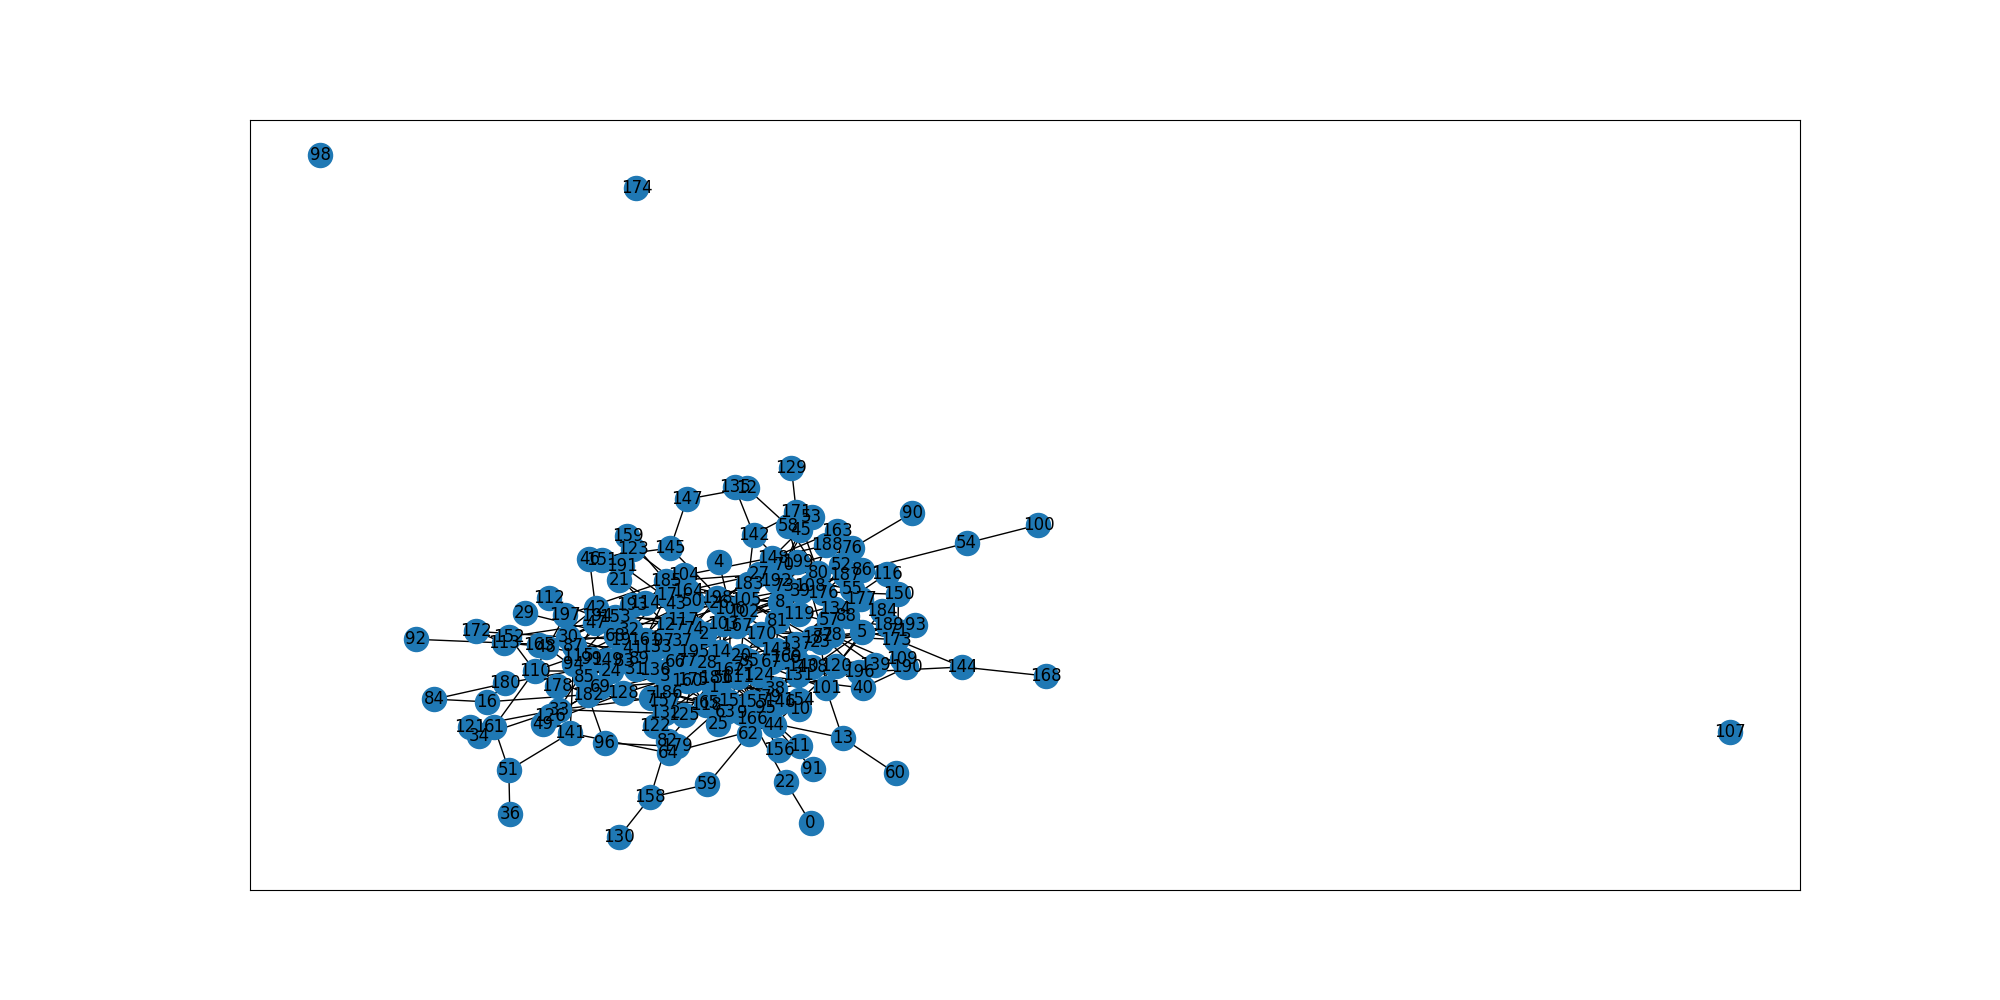
\includegraphics[width=\linewidth]{images/erdos_renyi/n200_p0.016491586832740178_0.png}
        \end{minipage}\hfill
        \begin{minipage}{0.32\textwidth}
            \centering
            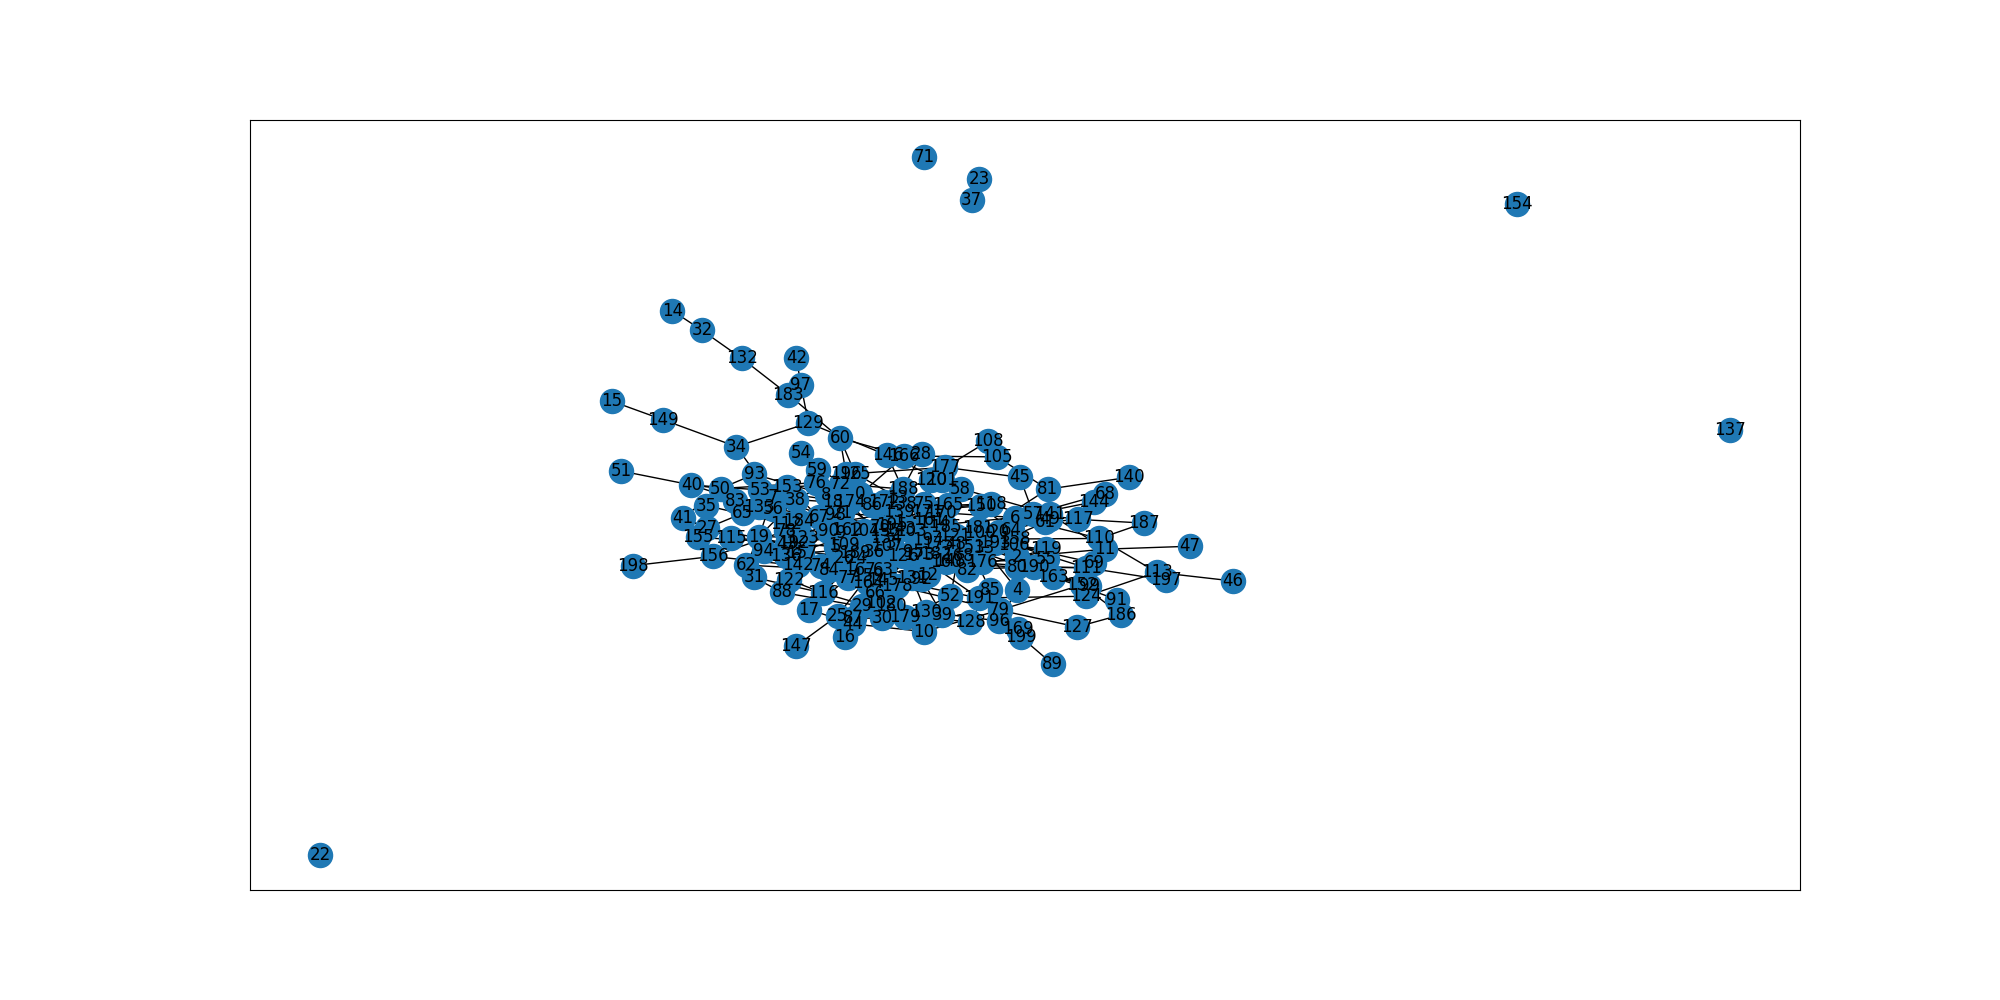
\includegraphics[width=\linewidth]{images/erdos_renyi/n200_p0.016491586832740178_1.png}
        \end{minipage}\hfill
        \begin{minipage}{0.32\textwidth}
            \centering
            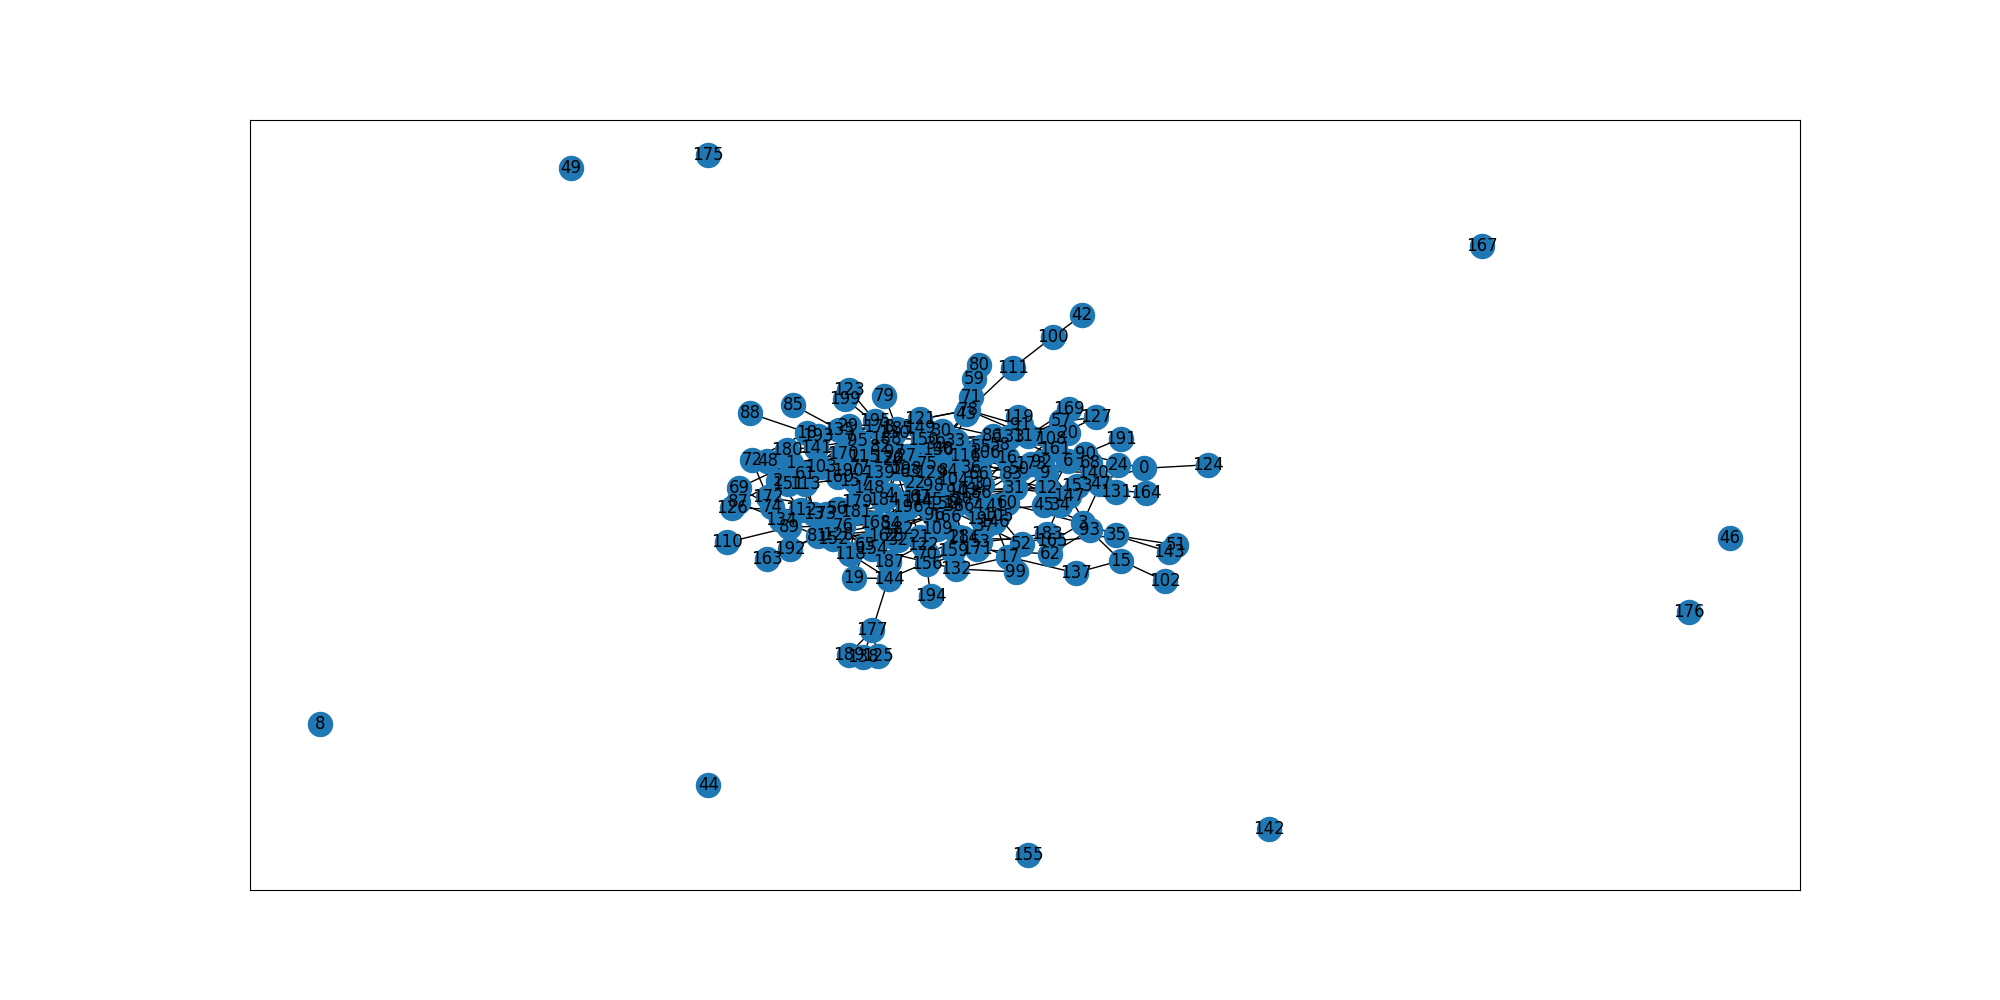
\includegraphics[width=\linewidth]{images/erdos_renyi/n200_p0.016491586832740178_2.png}
        \end{minipage}
        \caption{$n=200$, $p=0.01649$}
    \end{subfigure}

    \par\bigskip

    \begin{subfigure}{\textwidth}
        \centering
        \begin{minipage}{0.32\textwidth}
            \centering
            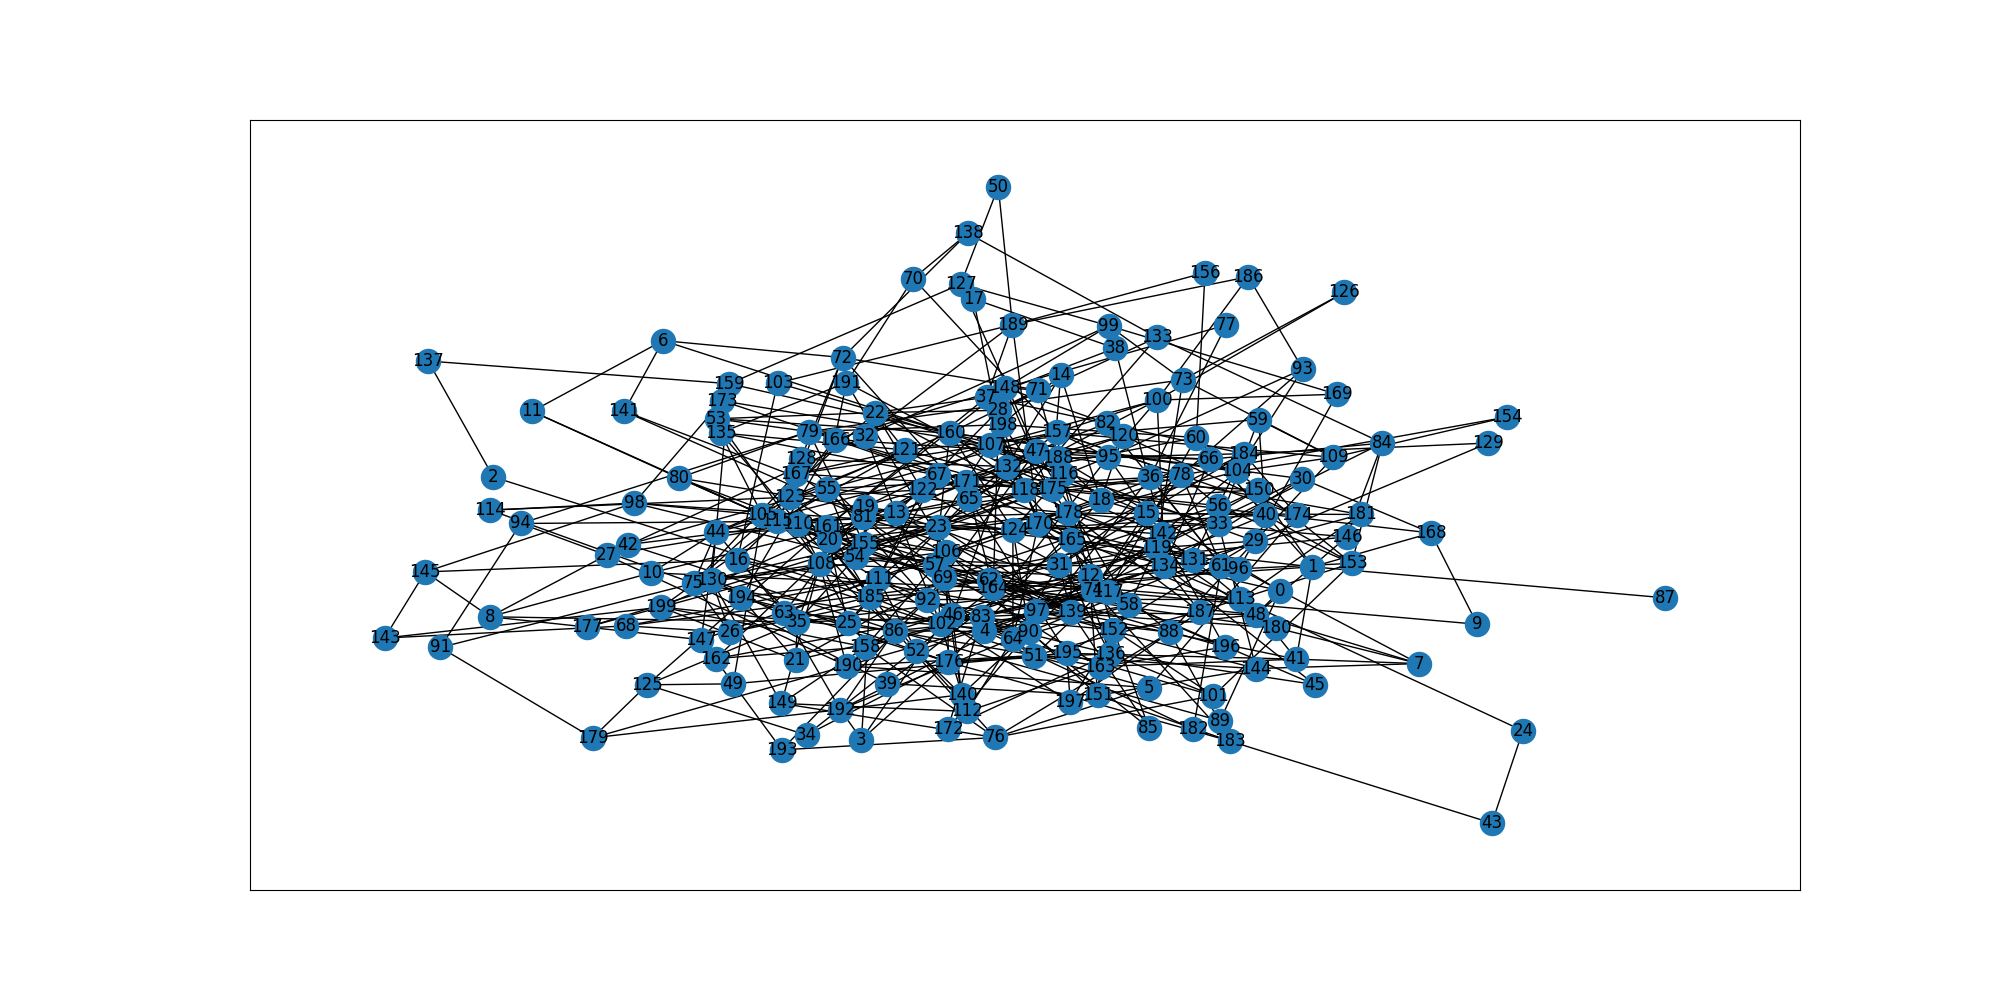
\includegraphics[width=\linewidth]{images/erdos_renyi/n200_p0.02649158683274018_0.png}
        \end{minipage}\hfill
        \begin{minipage}{0.32\textwidth}
            \centering
            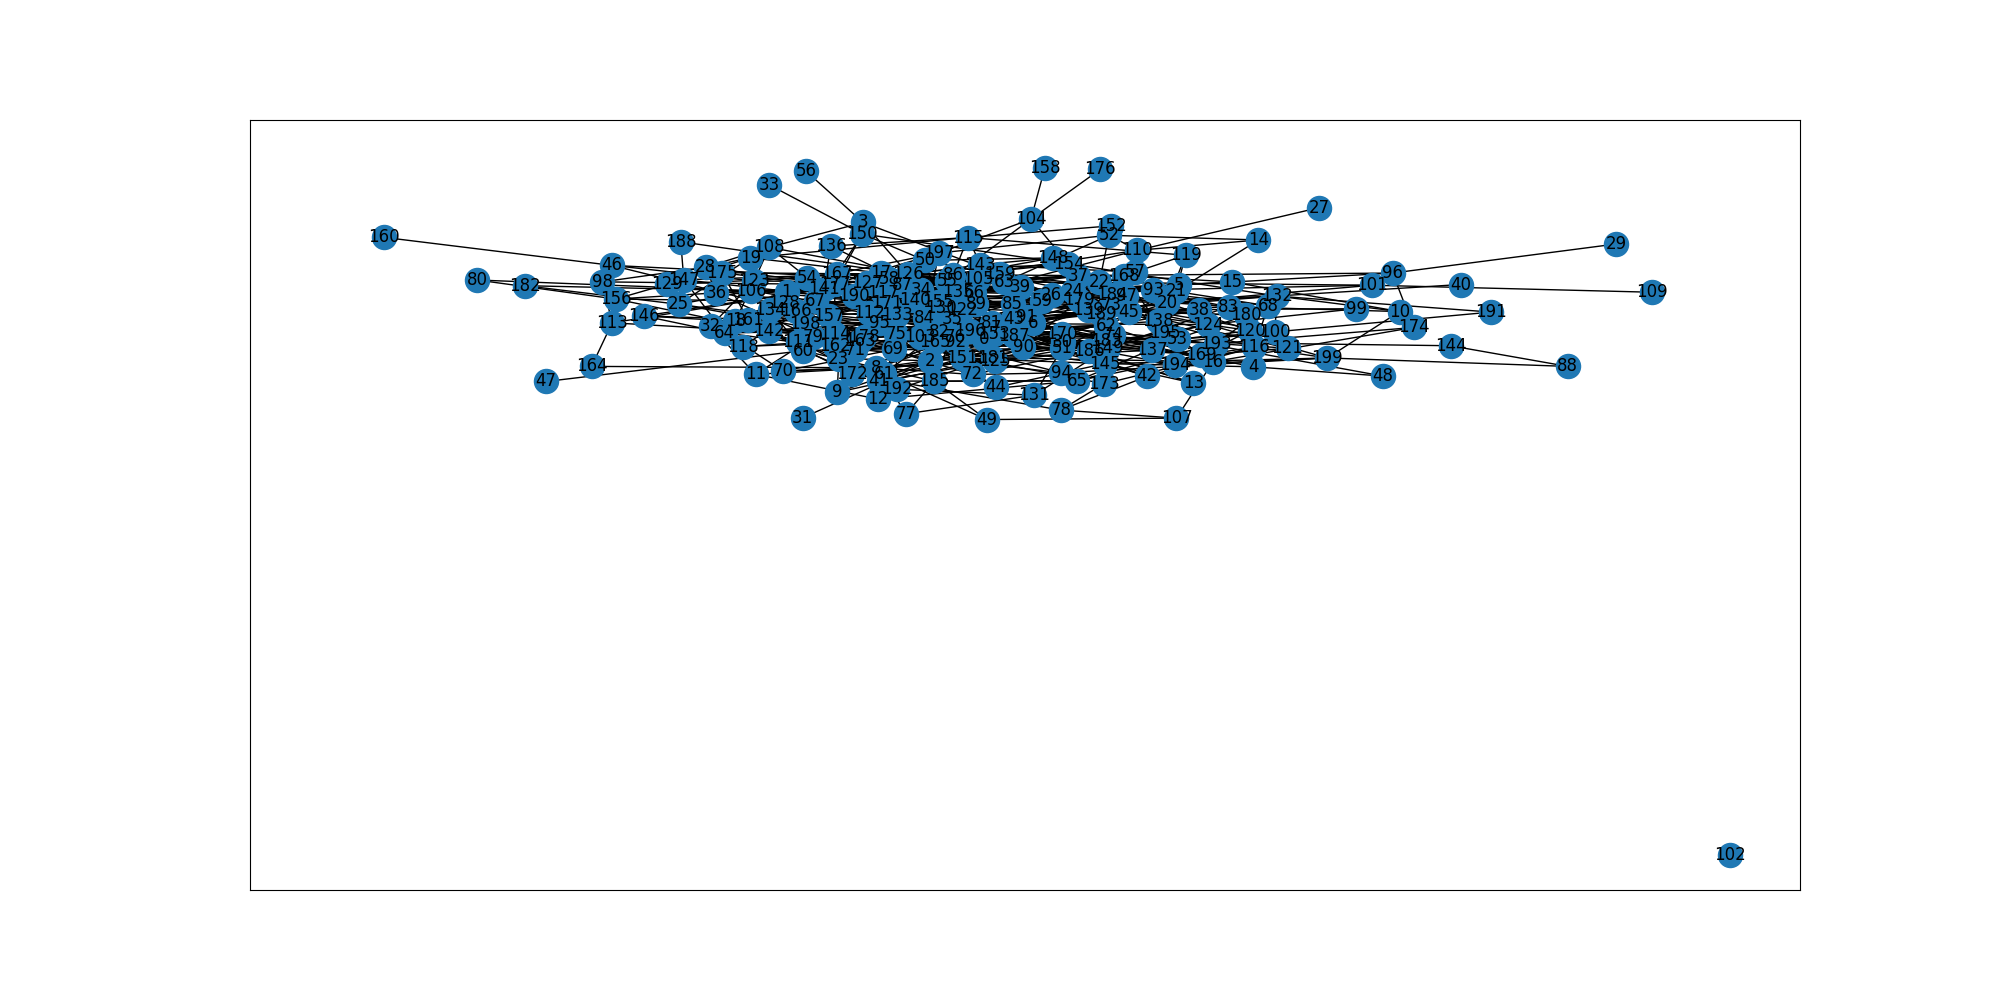
\includegraphics[width=\linewidth]{images/erdos_renyi/n200_p0.02649158683274018_1.png}
        \end{minipage}\hfill
        \begin{minipage}{0.32\textwidth}
            \centering
            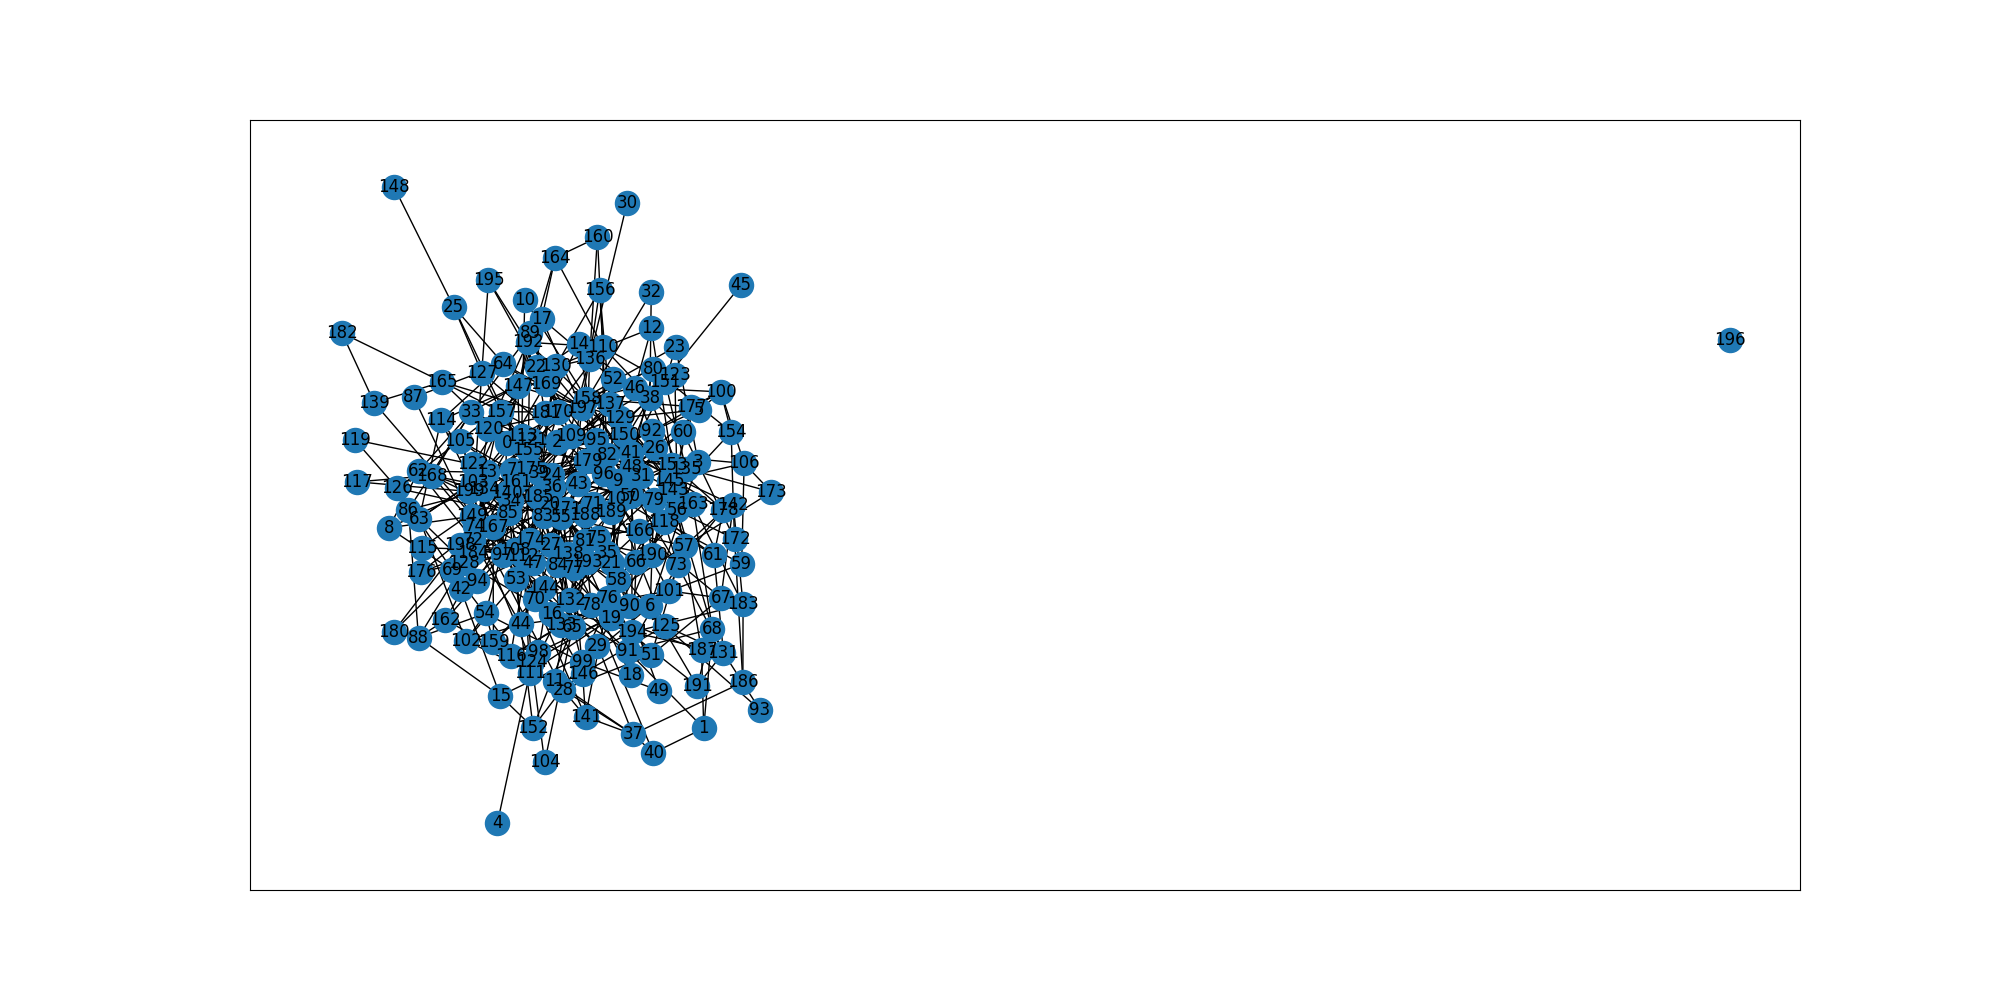
\includegraphics[width=\linewidth]{images/erdos_renyi/n200_p0.02649158683274018_2.png}
        \end{minipage}
        \caption{$n=200$, $p=0.02649$}
    \end{subfigure}

    \par\bigskip

    \begin{subfigure}{\textwidth}
        \centering
        \begin{minipage}{0.32\textwidth}
            \centering
            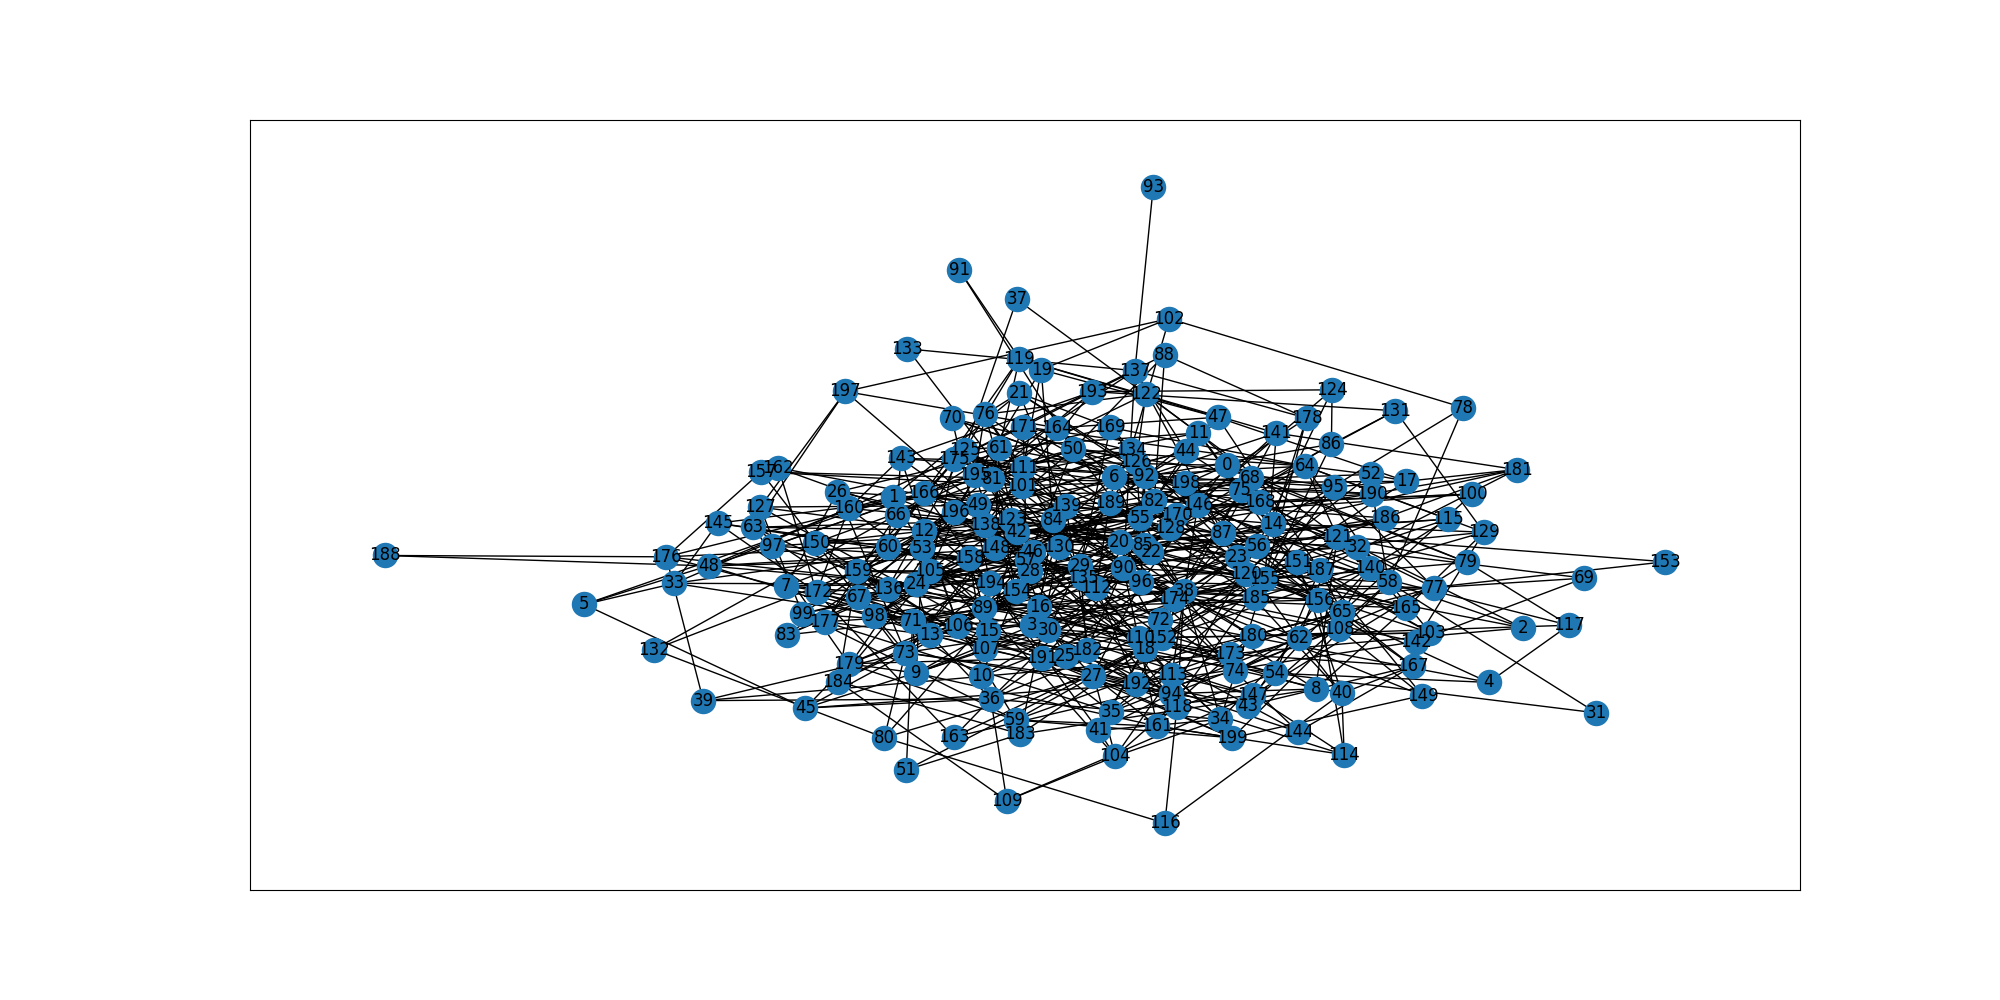
\includegraphics[width=\linewidth]{images/erdos_renyi/n200_p0.03649158683274018_0.png}
        \end{minipage}\hfill
        \begin{minipage}{0.32\textwidth}
            \centering
            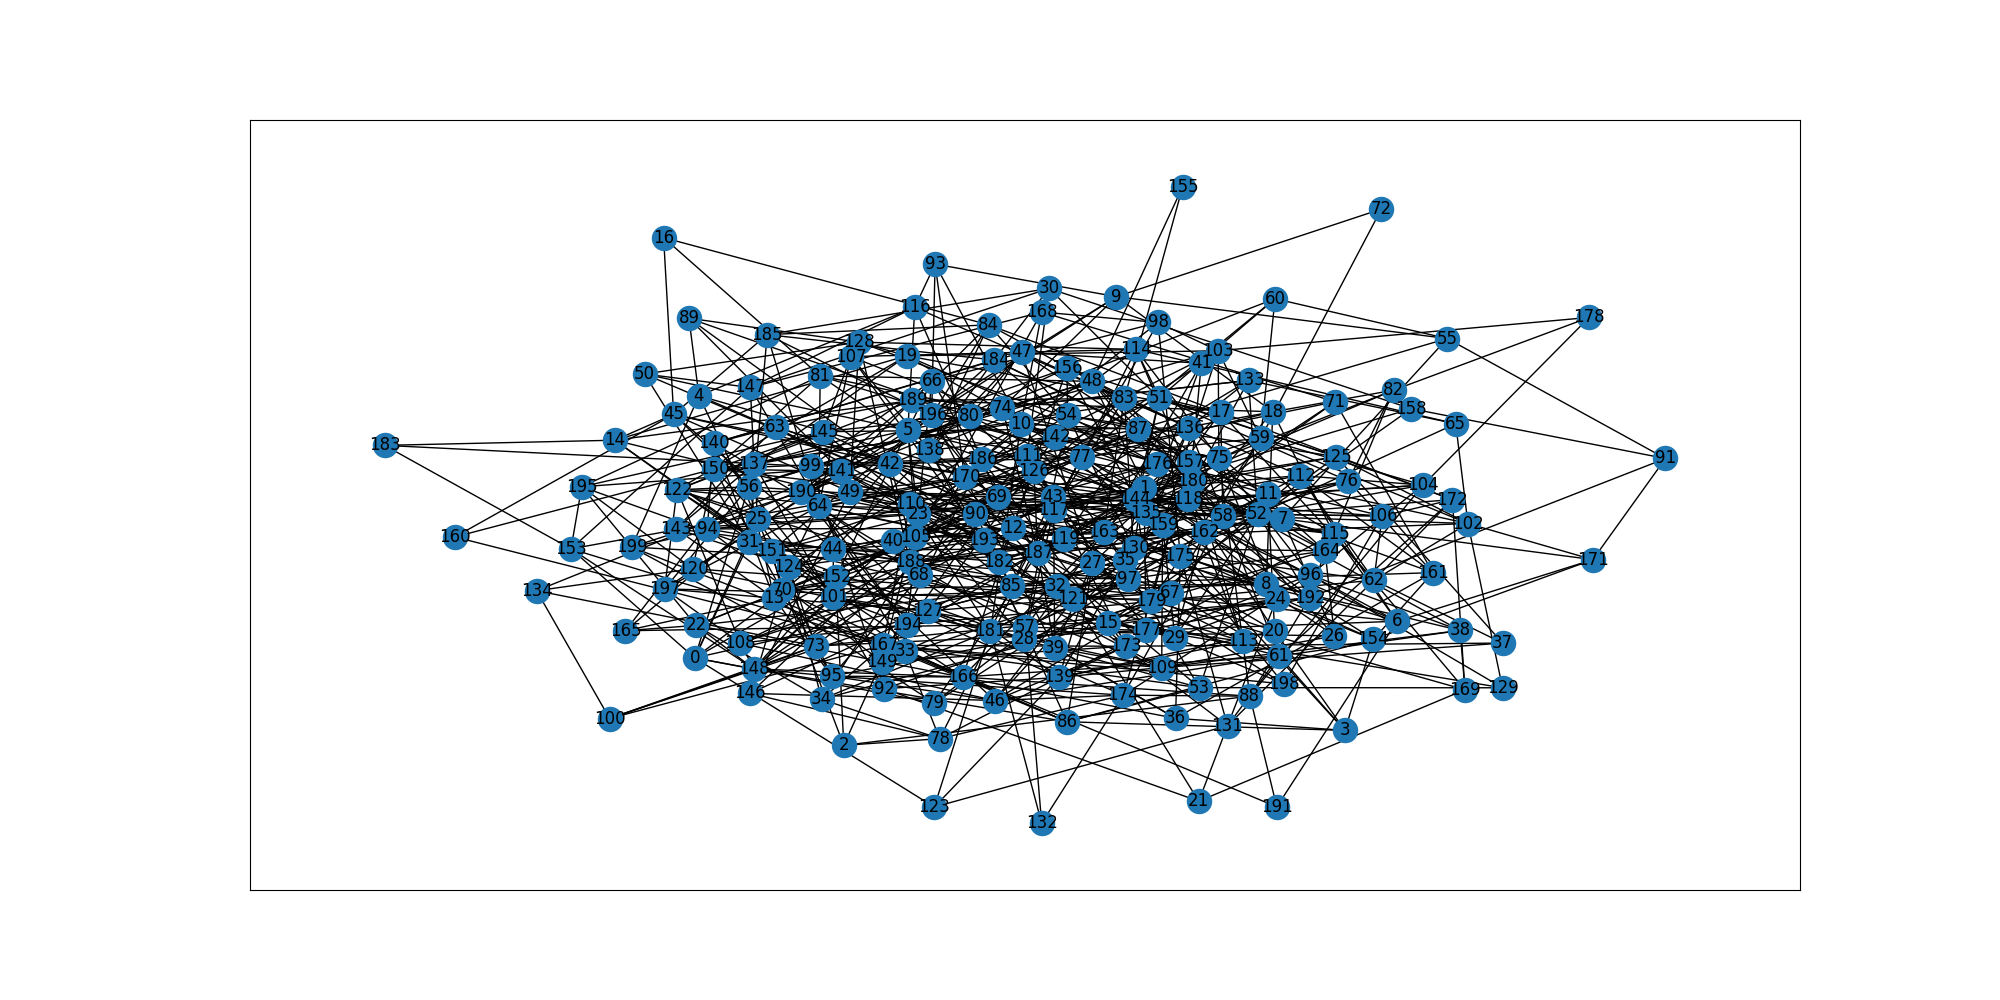
\includegraphics[width=\linewidth]{images/erdos_renyi/n200_p0.03649158683274018_1.png}
        \end{minipage}\hfill
        \begin{minipage}{0.32\textwidth}
            \centering
            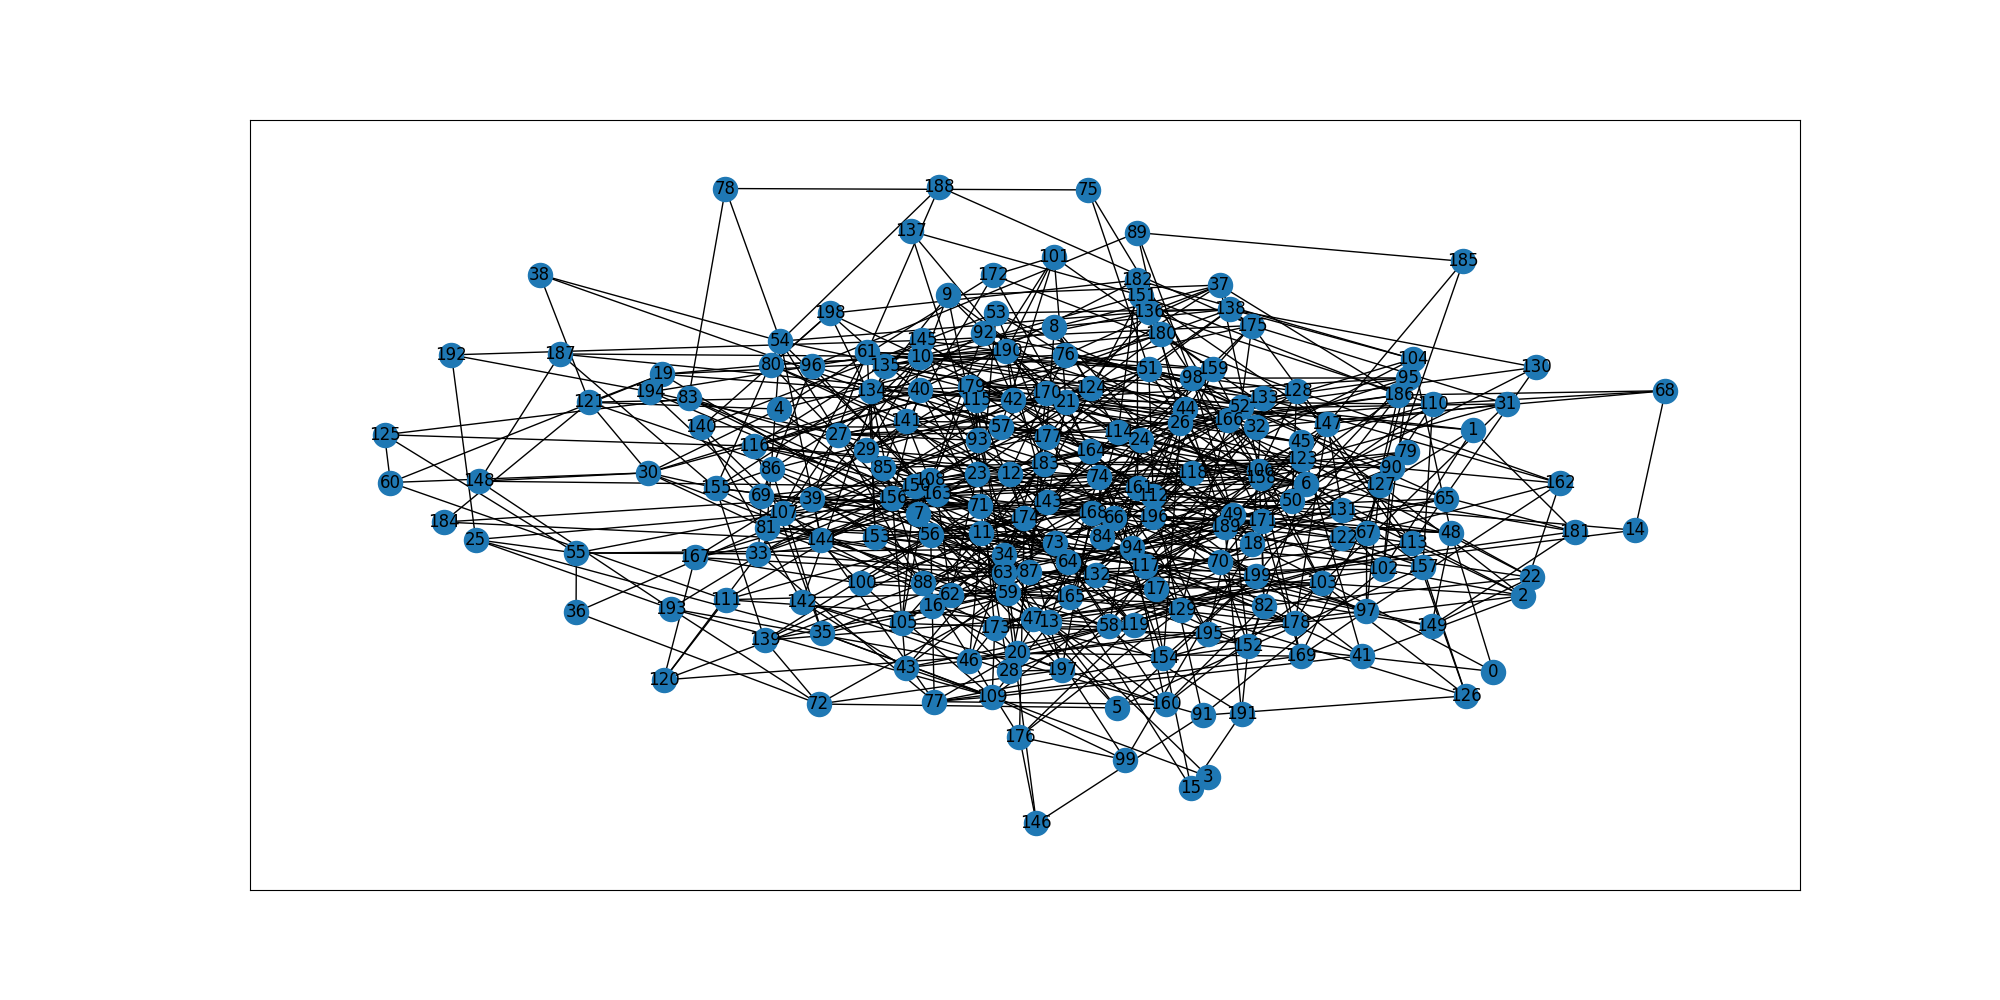
\includegraphics[width=\linewidth]{images/erdos_renyi/n200_p0.03649158683274018_2.png}
        \end{minipage}
        \caption{$n=200$, $p=0.03649$}
    \end{subfigure}

    \caption{Nueve realizaciones de grafos ER con $n=200$ y tres valores de $p$ alrededor del umbral de conectividad $p \approx \ln(n)/n$: fila 1 $p=0.01649$, fila 2 $p=0.02649$, fila 3 $p=0.03649$.}
    \label{fig:er_threshold}
\end{figure}

En la figura~\ref{fig:er_threshold} hacemos una validación empírica de esta propiedad, generando nueve grafos
con el algoritmo de ER con 200 nodos, variando la probabilidad $p$ alrededor del umbral de conectividad $p \approx \ln(n)/n \approx 0.02649$. Para cada valor de $p$ se generan tres grafos distintos.

La primera observación es que para valores de $p$ menores que el umbral de conectividad, el grafo es siempre disconexo, mientras que para valores de $p$ mayores que el umbral de conectividad, el grafo es siempre conexo. Cabe recalcar que las condiciones de las cotas~\eqref{eq:er_threshold_1} y~\eqref{eq:er_threshold_2} son probabilísticas, por lo que puede existir una realización del grafo que no cumpla con la condición, solo
que esto es altamente improbable. En el caso que $p$ es igual al umbral de conectividad, no podemos afirmar ningún comportamiento, y se ve reflejado en que algunos de los grafos son conexos y otros no. 

Otra característica a destacar, es que cuando el grafo ER no es conexo, las componentes que no pertenecen
a la componente conexa más grande, son nodos aislados. Esto esta relacionado a la tendencia de los grafos ER
a tener una componente gigante cuando $np>1$, condición que cumplen las 3 probabilidades elegidas.

\section{Grafos SBM}

\section{Grafos RDPG}

\subsection{definicion}

\subsection{inferencia}

\subsection{Clustering }

\section{Ejemplo real}

\bibliographystyle{plain}
\bibliography{refs}

\end{document}